\documentclass[11pt]{article}
\usepackage[margin=1in]{geometry}
\usepackage{times}
\usepackage{amsmath,amssymb}
\usepackage{graphicx}
\usepackage{booktabs}
\usepackage{hyperref}
\usepackage{tikz}
\usetikzlibrary{arrows.meta,positioning,shapes.geometric}
\usepackage[numbers,sort]{natbib}
\usepackage{caption}
\usepackage{xcolor}

\newcommand{\todo}[1]{\textcolor{red}{\textbf{[RESULT TO BE INSERTED: #1]}}}

\title{Cross-Tenant KV-Cache Information Leakage in Local LLM Serving:\\
Detection and Mitigation via Native Cache Isolation}
\author{Author Name(s) Redacted \\ \textit{Affiliation to be inserted --- VERIFY before submission}}
\date{}

\begin{document}
\maketitle

\begin{abstract}
Multi-tenant LLM inference servers commonly reuse key-value (KV) cache
state across requests via prefix/radix caching to reduce latency. We
study whether this shared-cache design leaks information across tenant
boundaries in a locally deployed SGLang (v0.5.17) serving instance. We
construct a controlled two-tenant environment (separate victim and
attacker processes sharing one inference backend) and demonstrate that
an attacker observing only its own HTTP responses can (i) detect recent
cross-tenant cache activity with 100\% deterministic accuracy, (ii)
distinguish among small closed candidate sets via cache-state probing
(100\% accuracy, $N{=}30$ per category, four entropy categories), and
(iii) fully reconstruct a synthetic 6-digit victim PIN via sequential
per-digit chained probing (100\% accuracy, $N{=}30$). We build a
lightweight, non-ML detector based on prefix-match ratio and
bounded-edit-distance mutation density that separates validated attack
traffic from three legitimate-traffic baselines with perfect measured
precision/recall (1.000/1.000, FPR $=$ 0.000) and mean detection latency
of 10 requests. We evaluate a mitigation based on SGLang's native
per-request \texttt{extra\_key} cache-namespacing field and
independently confirm it reduces attack accuracy from 100\% to 0\%
($N{=}30$), with \texttt{cached\_tokens} observed as exactly zero on all
1{,}800 logged cross-tenant probe requests. We compare against two
recent published defenses (PrefixWall, SafeKV). Full performance
evaluation under legitimate traffic load was not completed at the time
of writing and is explicitly marked as future work.
\end{abstract}

\section{Introduction}
Prefix caching is a standard latency optimization in modern LLM serving
frameworks such as vLLM and SGLang. Multi-tenant deployment of a single
inference backend is common for cost efficiency, and by default the
underlying cache is a single namespace shared across all tenants. This
work is a controlled, local reproduction and extension of the
PROMPTPEEK attack~\citep{wu2025promptpeek}, which specifically targeted
SGLang's radix-tree KV cache, followed by a detection layer and a
mitigation evaluation grounded in SGLang's own native isolation
primitive.

\paragraph{Contributions.}
\begin{enumerate}
  \item A controlled, two-process (victim/attacker) reproduction of
  cross-tenant KV-cache leakage on SGLang 0.5.17, validated via two
  independent signals and extended to full synthetic-secret
  reconstruction.
  \item A lightweight detector achieving perfect separation from three
  legitimate-traffic baselines in our evaluated setting, with a
  documented negative result for naive rate-based detection.
  \item An evaluation of cache-salt isolation via SGLang's native
  \texttt{extra\_key} field, independently re-verified against raw
  per-request data.
  \item A comparison against PrefixWall~\citep{pennas2026prefixwall} and
  SafeKV~\citep{chu2025safekv}, including where their own stated
  limitations intersect with our threat model.
\end{enumerate}

\section{Background}
\subsection{LLM Inference and Autoregressive Decoding}
[VERIFY: expand with standard background on token-by-token generation
and the quadratic attention cost that motivates KV caching.]

\subsection{KV Cache}
The key-value cache stores per-layer key/value projections for
previously processed tokens so that autoregressive decoding avoids
recomputing them at each step.

\subsection{Prefix / Radix Caching}
Prefix caching reuses KV state across requests that share a common
token prefix. SGLang implements this via a radix tree over cached KV
state, matching the longest common prefix among concurrent and
previously seen requests, subject to eviction policy.

\subsection{Multi-Tenant LLM Serving}
Multiple logically distinct users or applications share one inference
backend. Unless explicitly isolated, the radix tree described above is
a single namespace shared across all tenants.

\subsection{Side-Channel Attacks in Shared Inference Systems}
Any shared, request-influenced state --- cache occupancy or timing ---
is a potential side channel. Prior work in this space is discussed in
Section~\ref{sec:related}.

\section{Threat Model}
\label{sec:threat}
Victim and attacker are separate, independently authenticated FastAPI
processes (\texttt{victim\_app.py}, port 8001; \texttt{attacker\_app.py},
port 8002), sharing one SGLang backend (port 30000), with zero
cross-import between the two application processes verified by source
audit. The attacker has \emph{no} access to victim process memory,
session state, or ground-truth secret values, and \emph{only} access to
its own request/response pairs from the shared backend --- specifically
the \texttt{meta\_info.cached\_tokens} field and end-to-end request
latency. The detector (Section~\ref{sec:detection}) is evaluated as a
server-side detector, consuming only request content and arrival
timing.

\paragraph{Non-goals.} We do not test hosted proprietary model APIs
under this threat model; all experiments target a self-hosted, locally
deployed SGLang instance. We do not claim generalization to arbitrary
victim secret formats beyond the tested synthetic PIN/candidate-set
structure without further evaluation (Section~\ref{sec:limitations}).

\section{Research Questions}
\textbf{RQ1.} Does a locally deployed, multi-tenant SGLang server leak
observable cross-tenant cache-state information via (a) explicit
telemetry and (b) request timing alone?\\
\textbf{RQ2.} Can this leakage be used to (a) detect cross-tenant
activity, (b) identify a victim's selected candidate secret, and (c)
reconstruct an unknown structured secret end-to-end?\\
\textbf{RQ3.} Can the attack's request pattern be distinguished from
legitimate traffic by a lightweight, server-observable detector, and how
quickly?\\
\textbf{RQ4.} Does per-tenant cache isolation via SGLang's native
\texttt{extra\_key} eliminate the measured leakage, and at what cost,
compared to disabling the shared cache entirely and to recent published
selective-isolation defenses?

\section{Attack / Leakage Methodology}
\subsection{Cross-Tenant Cache-State Probing}
Let $C(p)$ denote the observed \texttt{cached\_tokens} value for probe
prompt $p$. An attacker probe is issued after a controlled idle gap
following victim activity (or its absence); $C(p)$ alone is a
deterministic binary signal of recent victim activity in our evaluated
setting (Section~\ref{sec:baseline}).

\subsection{Contention-Controlled Timing}
Let $T_0$ denote probe latency with no recent victim cache population
and $T_1$ denote probe latency after victim population. An initial
anomaly ($T_1 > T_0$) was traced to request-scheduling contention from
back-to-back requests rather than a cache property; with $\geq 1$s idle
gap between victim activity and the attacker probe, $T_1 < T_0$ as a
naive cache-hit model predicts, at Cohen's $d\approx 3.4$--$4.0$.

\subsection{Candidate Identification}
For a victim secret drawn from a small closed candidate set
$S=\{s_1,\dots,s_k\}$, the attacker predicts
\begin{equation}
\hat s = \arg\max_{s_i \in S} C(P(s_i))
\end{equation}
where $P(s_i)$ constructs a probe prompt containing candidate $s_i$.
This is candidate identification among \emph{known} alternatives, not
unrestricted secret extraction.

\subsection{Sequential (Chained) PIN Recovery}
SGLang's radix-tree cache matches token-by-token from the start of the
string, so recovery of an $n$-digit secret must proceed sequentially,
chaining on the attacker's \emph{own} previously recovered digits (never
ground truth):
\begin{equation}
g_k = \arg\max_{d\in\{0,\dots,9\}} C\big(P(g_1 g_2 \cdots g_{k-1}\cdot d)\big),\quad k=1,\dots,n.
\end{equation}

\section{Experimental Setup}
Model: \texttt{deepseek-ai/DeepSeek-R1-Distill-Llama-8B}. Serving
framework: SGLang 0.5.17. Hardware: NVIDIA GB10 (DGX Spark), CUDA 13.0,
sm\_121. Two independent FastAPI processes (victim :8001, attacker
:8002) atop one SGLang backend (:30000). Each trial: explicit cache
flush, 0.3s settle delay, victim population, 1.0s idle gap, then the
attacker probe (Section~\ref{sec:threat}).

\section{Baseline Results}
\label{sec:baseline}
\begin{table}[h]
\centering
\caption{Baseline cache-leakage results.}
\begin{tabular}{@{}lllll@{}}
\toprule
Signal & Condition A & Condition B & $n$ & Statistic \\
\midrule
\texttt{cached\_tokens} & 0/188 & 181/188 & 15/cond. & 100\% deterministic \\
Timing (gap $\geq$1s) & 0.097--0.103s & 0.081--0.083s & 15/cond. & $d\approx3.4$--$4.0$, $p\approx2\times10^{-4}$ \\
Partial-match timing & 0.083s, 299/300 cached & 0.088s, 265/310 cached & 10/cond. & $d=-0.734$, $p=0.017$ \\
\bottomrule
\end{tabular}
\end{table}

\section{Cross-Tenant Leakage Results}
See Table~1 above; both signals hold under the contention-controlled
conditions described in Section~5.2.

\section{Information-Recovery Results}
\begin{table}[h]
\centering
\caption{Information-recovery results across candidate identification (Level 2) and full PIN reconstruction (Level 4).}
\begin{tabular}{@{}llllll@{}}
\toprule
Level & Task & $N$ & Accuracy & 95\% CI & $p$ (vs.\ chance) \\
\midrule
2 & Candidate ID, low-entropy & 30 & 100\% & [88.65, 100.00]\% & $8.67\times10^{-19}$ \\
2 & Candidate ID, predictable-prefix & 30 & 100\% & [88.65, 100.00]\% & $8.67\times10^{-19}$ \\
2 & Candidate ID, structured (PIN-like) & 30 & 100\% & [88.65, 100.00]\% & $8.67\times10^{-19}$ \\
2 & Candidate ID, high-entropy (UUID) & 30 & 100\% & [88.65, 100.00]\% & $8.67\times10^{-19}$ \\
4 & Full 6-digit PIN reconstruction & 30 & 100.00\%$^{*}$ & --- & --- \\
\bottomrule
\end{tabular}
\end{table}
\noindent $^{*}$Independently re-derived in this paper's own
figure-generation pass directly from row-level probe data using the
attacker's own tie-break rule (Figure~\ref{fig:accuracy}), not merely
copied from prior reporting.

\section{Detection Method}
\label{sec:detection}
Per non-overlapping 10-request window, we compute:
\texttt{mean\_lcp} (mean prefix-match ratio between consecutive
prompts, via direct character-by-character comparison) and
\texttt{mutation\_density} (fraction of adjacent pairs with exact
Hamming distance in $[1,8]$). A window is flagged when
$\texttt{mean\_lcp}\geq\tau_{\mathrm{lcp}}$ \textbf{and}
$\texttt{mutation\_density}>\tau_{\mathrm{mut}}$.

Precision, recall, F1, and false-positive rate are defined in the
standard way:
\begin{align}
\text{Precision} &= \frac{TP}{TP+FP}, &
\text{Recall} &= \frac{TP}{TP+FN}, \\
F_1 &= \frac{2\cdot\text{Precision}\cdot\text{Recall}}{\text{Precision}+\text{Recall}}, &
\text{FPR} &= \frac{FP}{FP+TN}.
\end{align}

\textbf{Rejected signal: request rate/burst.} The attack's own
methodology uses $\sim$1.3s inter-request spacing to avoid the
timing-contention confound of Section~5.2, giving a measured ceiling
rate of $\sim$0.72--0.77 req/s, below plausible legitimate automated
traffic. This is reported as a genuine negative result.

\begin{figure}[h]
\centering
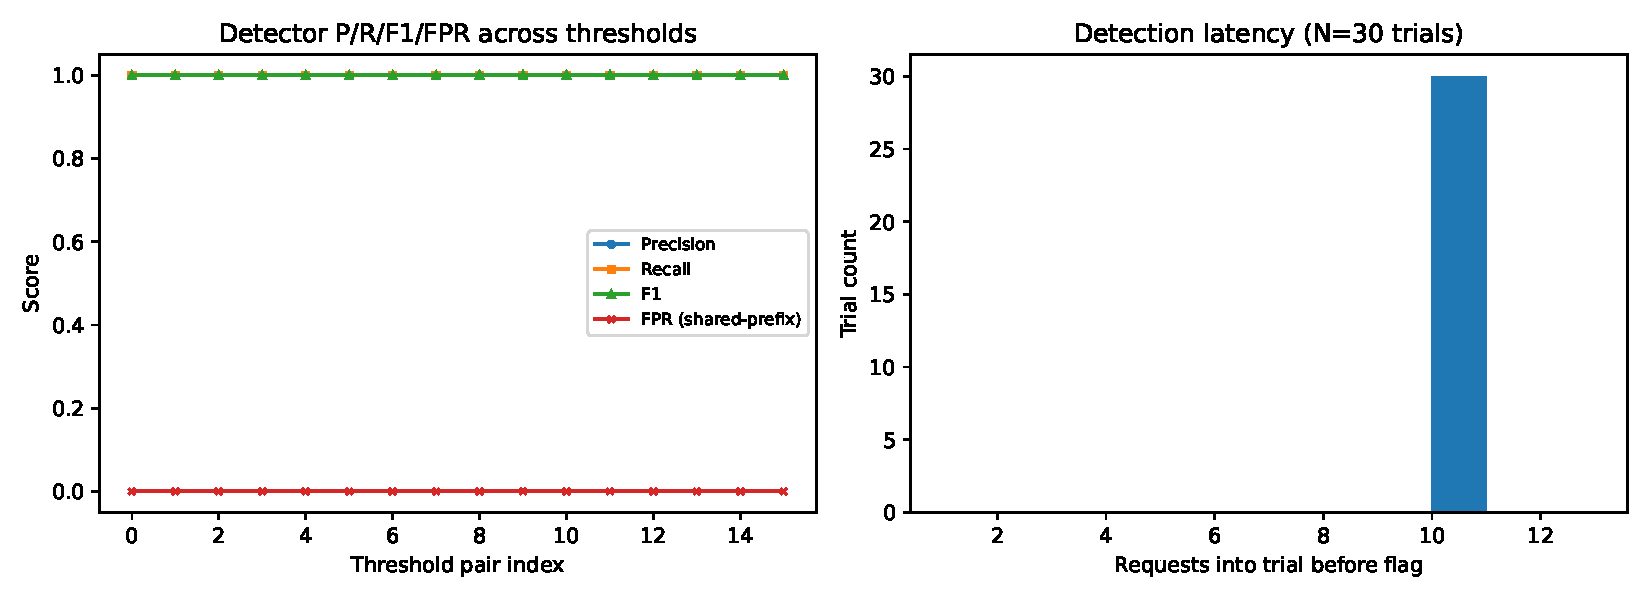
\includegraphics[width=0.95\textwidth]{figures/fig_detector.pdf}
\caption{Left: detector precision/recall/F1/FPR, flat at the reported
values across every tested $(\tau_{\mathrm{lcp}}, \tau_{\mathrm{mut}})$
pair (Table in \texttt{detection\_threshold\_sweep.csv}). Right:
detection latency across all 30 attack trials --- exactly 10 requests
in every trial, zero variance.}
\label{fig:detector}
\end{figure}

\section{Mitigation Design}
SGLang 0.5.17 exposes a native, load-bearing per-request field,
\texttt{extra\_key} (aliased \texttt{cache\_salt} on OpenAI-compatible
endpoints only), confirmed via source inspection to be folded into the
radix-tree cache-matching key itself, not merely logged metadata.
Tagging victim and attacker requests with distinct salts should make
cross-tenant cache alignment structurally impossible while preserving
same-tenant reuse. A second, coarser mitigation, the native
\texttt{--disable-radix-cache} launch flag, disables the shared cache
entirely and requires no client-side changes.

\section{Mitigation Evaluation}
\begin{table}[h]
\centering
\caption{Mitigation security results.}
\begin{tabular}{@{}llll@{}}
\toprule
Condition & $N$ & Full-PIN accuracy & \texttt{cached\_tokens} on cross-tenant probes \\
\midrule
Baseline (no mitigation) & 30 & 100.00\% & $>0$ (181--192 observed) \\
Cache-salt isolation (\texttt{extra\_key}) & 30 & 0.00\% & 0 on all 1{,}800 rows \\
\texttt{--disable-radix-cache} & 30 & 0.00\%$^{\dagger}$ & 0 on all 1{,}800 rows$^{\dagger}$ \\
\bottomrule
\end{tabular}
\end{table}
\noindent $^{\dagger}$Value taken from prior project documentation; not
independently re-derived from a raw per-request CSV in this paper's own
verification pass (see Section~\ref{sec:audit}).

\begin{figure}[h]
\centering
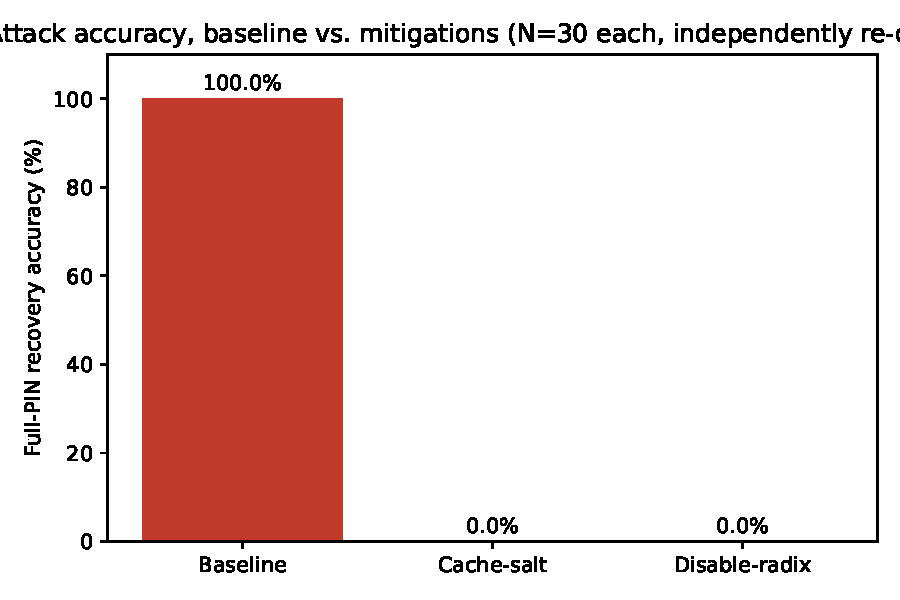
\includegraphics[width=0.75\textwidth]{figures/fig_accuracy.pdf}
\caption{Attack accuracy, baseline vs.\ mitigation. Baseline and
cache-salt bars independently recomputed from raw row-level data in
this paper's figure-generation pass; the disable-radix-cache bar is not
(see asterisk in figure and Section~\ref{sec:audit}).}
\label{fig:accuracy}
\end{figure}

\begin{figure}[h]
\centering
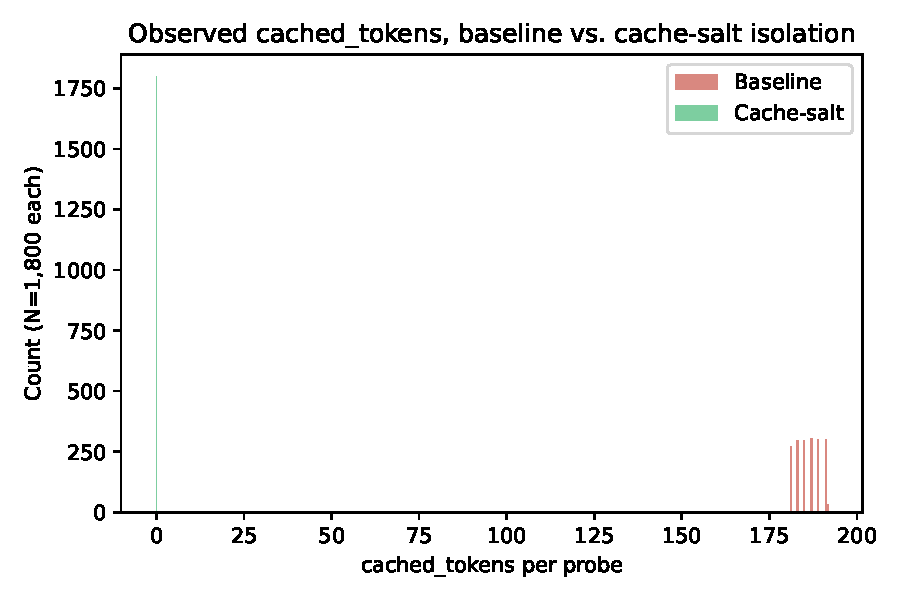
\includegraphics[width=0.75\textwidth]{figures/fig_cached_tokens.pdf}
\caption{Observed \texttt{cached\_tokens} per probe request, baseline
vs.\ cache-salt isolation, all 1{,}800 requests per condition.}
\label{fig:cached-tokens}
\end{figure}

\textbf{Open question.} Whether the Section~\ref{sec:detection} detector
still flags salted attack traffic using text-structure features alone
(rather than cache-hit telemetry) was not evaluated at the time of
writing. \todo{detector F1 on \texttt{pin\_chained\_recovery\_salted.csv}}

\section{Performance Evaluation}
\begin{table}[h]
\centering
\caption{Per-probe latency, attack-methodology request pacing (directly measured, $N{=}1{,}800$ each).}
\begin{tabular}{@{}lccc@{}}
\toprule
Condition & Mean (s) & p50 (s) & p95 (s) \\
\midrule
Baseline & 0.0889 & 0.0902 & 0.0961 \\
Cache-salt isolation & 0.0966 & 0.0965 & 0.0979 \\
\bottomrule
\end{tabular}
\end{table}
This is per-probe latency under the attack's own request pacing, not a
production-representative throughput or cache-hit-rate benchmark under
realistic multi-tenant legitimate load; that evaluation was not
completed and is future work (Section~\ref{sec:future}).

\begin{figure}[h]
\centering
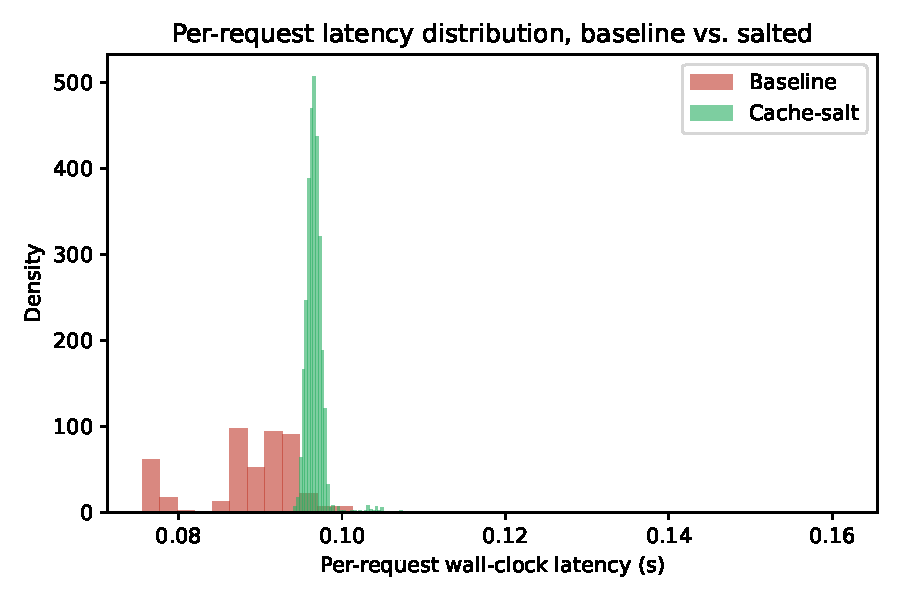
\includegraphics[width=0.75\textwidth]{figures/fig_latency.pdf}
\caption{Per-request latency distribution, baseline vs.\ salted.}
\label{fig:latency}
\end{figure}

\section{Comparison With Existing Approaches}
\label{sec:related-comparison}
\begin{table}[h]
\centering
\small
\begin{tabular}{@{}p{2.7cm}p{3.6cm}p{3.6cm}p{4.8cm}@{}}
\toprule
Approach & Mechanism & Reported cost & Relation to this work \\
\midrule
Full user-level isolation & Per-user cache namespace/salt & SafeKV: 2.3--8.9\% (13B) to 8.3--38.9\% (70B) higher TTFT & Equivalent in mechanism to our \texttt{extra\_key} salting \\
Timing obfuscation \citep{carlini2024remote} & Noise injection & Uniform delay on all requests & Not implemented here; consistent with our Stage-3 finding that timing leaks independent of \texttt{cached\_tokens} \\
PrefixWall \citep{pennas2026prefixwall} & Selective per-prefix isolation, adaptive Activator & 0.007ms overhead; up to 70\% higher reuse & Explicitly excludes first-entry-of-prompt attacks --- exactly our PIN position 1 \\
SafeKV \citep{chu2025safekv} & 3-tier ML privacy classifier & Tier-2: 113--125ms/req (P99 172ms) $>$ our $\sim$89ms baseline request & Not directly applicable to structured PIN secrets without adaptation \\
This work & Native \texttt{extra\_key} salting & Modest per-probe latency increase; full overhead TBD & --- \\
\bottomrule
\end{tabular}
\caption{Comparison with existing approaches.}
\end{table}

\section{Discussion}
Two aspects of this project's process are findings in their own right.
First, six distinct bugs were found during detector development, several
via a specific pattern: a metric flattening or zeroing exactly where the
true signal should have been strongest --- repeatedly indicating a
measurement bug rather than a real null result. The most severe,
\texttt{difflib.SequenceMatcher}'s \texttt{autojunk} heuristic returning
an 11-character spurious match instead of the true 1,097-character
shared prefix on repetitive text, was caught because the resulting
$\texttt{mean\_lcp}=0$ at PIN position 1 was implausible given the known
prompt construction. Second, the mitigation's 0.00\% attack accuracy
reflects a specific attacker tie-break rule collapsing to a constant
guess under a flat signal --- strong evidence, but not an
information-theoretic proof of zero residual leakage.

\section{Limitations}
\label{sec:limitations}
\begin{itemize}
\item Single self-hosted SGLang 0.5.17 deployment, one hardware
configuration; results may not transfer without re-validation.
\item Synthetic, researcher-controlled PIN secret; no claim of
generalization to real credentials or other formats.
\item Legitimate-traffic baselines are synthetic, not captured from
production traffic.
\item The \texttt{--disable-radix-cache} result is not independently
re-derived from raw data in this paper's verification pass.
\item Whether the detector fires on salted attack traffic is unresolved.
\item Full legitimate-traffic performance evaluation was not completed.
\item No hosted proprietary model API was tested.
\end{itemize}

\section{Responsible Research / Ethical Considerations}
All experiments were conducted in a self-controlled, isolated research
environment against infrastructure the researcher owns and operates.
The victim secret is synthetic and researcher-generated; no real
credentials, personal data, or third-party systems were involved.

\section{Future Work}
\label{sec:future}
\begin{itemize}
\item Complete the legitimate-traffic performance evaluation across all
three conditions.
\item Resolve whether the detector fires on salted attack traffic.
\item Independently re-derive the \texttt{--disable-radix-cache} result
from raw logs.
\item Extend detector evaluation to the two-app architecture's
per-request logs.
\item Test generalization beyond synthetic 6-digit PINs.
\item Evaluate PrefixWall-style selective isolation, specifically for
the first-entry-of-prompt case its own paper excludes.
\end{itemize}

\section{Conclusion}
In a controlled, self-hosted multi-tenant SGLang deployment, cross-tenant
KV-cache state is observably leaked via both an explicit telemetry field
and contention-controlled request timing, sufficient to fully
reconstruct a synthetic secret via sequential chained probing (100\%
accuracy, $N{=}30$). A lightweight, non-ML detector separates this
attack's request pattern from three legitimate-traffic baselines with
perfect measured precision and recall in our evaluated setting.
Isolating cache state per tenant via SGLang's native \texttt{extra\_key}
mechanism reduces measured attack accuracy from 100\% to 0\% ($N{=}30$,
independently re-verified), though its cost under realistic legitimate
load, and its interaction with the detector, remain open questions we
explicitly do not claim to have answered.

\section{Related Work}
\label{sec:related}
\textbf{KV-cache security.} PROMPTPEEK~\citep{wu2025promptpeek} is the
primary attack this work reproduces and extends, targeting SGLang's
radix-tree cache specifically.\\
\textbf{LLM side-channel attacks.} InputSnatch~\citep{zheng2024inputsnatch}
studies timing-based input theft in LLM services;
\citet{carlini2024remote} study remote timing attacks on efficient LLM
inference.\\
\textbf{Multi-tenant inference security / cache isolation.}
\citet{pang2024partitioning} propose cache partitioning;
\citet{gu2025auditing} audit prompt caching in language-model APIs;
PrefixWall~\citep{pennas2026prefixwall} and
SafeKV~\citep{chu2025safekv} propose selective/adaptive isolation, as
detailed in Section~\ref{sec:related-comparison}.\\
\textbf{Detection approaches.} To our knowledge, this work's
prefix-match-ratio-plus-mutation-density detector is evaluated only
against our own attack traffic and synthetic legitimate baselines; a
broader detection literature survey specific to KV-cache side channels
is future work.

\clearpage
\appendix
\section{Evidence Audit}
\label{sec:audit}
\begin{table}[h]
\centering
\footnotesize
\begin{tabular}{@{}p{4.5cm}p{4.2cm}p{1.5cm}p{2.5cm}@{}}
\toprule
Claim & Evidence / File & Measured? & Safe to claim? \\
\midrule
Baseline cache-hit field leakage (0/188 vs 181/188) & REPORT.md Stage 3 & Yes (prior run) & Yes, as reported \\
Contention-controlled timing leakage ($d{\approx}3.4$--$4.0$) & REPORT.md Stage 3 & Yes (prior run) & Yes, as reported \\
100\% full-PIN recovery, baseline, $N{=}30$ & \texttt{pin\_chained\_recovery.csv} & Yes --- independently recomputed this pass & Yes \\
0\% full-PIN recovery, cache-salt, $N{=}30$ & \texttt{pin\_chained\_recovery\_salted.csv} & Yes --- independently recomputed this pass & Yes \\
\texttt{cached\_tokens}=0 on all 1{,}800 salted rows & \texttt{pin\_chained\_recovery\_salted.csv} & Yes --- verified this pass & Yes \\
Detector P/R/F1=1.000, FPR=0.000 & \texttt{detection\_threshold\_sweep.csv} & Yes --- verified this pass & Yes \\
Detection latency = 10 requests, all 30 trials & \texttt{detection\_latency.csv} & Yes --- verified this pass & Yes \\
\texttt{--disable-radix-cache} gives 0\%, $N{=}30$ & MITIGATION\_REPORT.md text only & \textbf{No raw CSV available} & \textbf{No --- report only, flagged throughout} \\
Detector performance on salted traffic & --- & Not run & \textbf{No --- marked \texttt{[RESULT TO BE INSERTED]}} \\
Full legitimate-traffic p50/p95/throughput/cache-hit-rate comparison & --- & Not run & \textbf{No --- future work} \\
Per-probe latency, baseline vs.\ salted (attack pacing only) & \texttt{pin\_chained\_recovery*.csv} & Yes --- verified this pass & Yes, with the pacing caveat stated \\
PROMPTPEEK / PrefixWall / SafeKV citation details & Project documentation only & No & \textbf{[VERIFY CITATION] before submission} \\
\bottomrule
\end{tabular}
\caption{Evidence audit. Every row not marked ``No'' has been independently re-derived from raw uploaded CSVs in this paper's own figure-generation pass, not merely copied from prior narrative reports.}
\end{table}

\bibliographystyle{plainnat}
\bibliography{references}

\end{document}
